\documentclass[11pt]{article}
%%%%%%%%% options for the file macros.tex
\usepackage[utf8]{inputenc}
\usepackage{savesym}
\usepackage{wrapfig}
% \usepackage{times}
\usepackage[dvipsnames]{xcolor}
\usepackage[ruled,vlined,linesnumbered, algo2e]{algorithm2e}
\usepackage{algpseudocode}
\renewcommand{\thealgocf}{}

\def\showauthornotes{1}
\def\showkeys{0}
\def\showdraftbox{0}
% \allowdisplaybreaks[1]
\savesymbol{nl}
%% Shamelessly adapted from a scribe template by Sanjeev Arora

%%%%%%%%%%%%%% Packages
% \usepackage[active,tightpage]{preview}
% \renewcommand{\PreviewBorder}{1in}
\usepackage[hidelinks]{hyperref}
\usepackage{amsmath,amssymb,amsthm,amstext,amsfonts,bbm,algorithm,algorithmicx,xspace,nicefrac,
  algpseudocode}
\usepackage{color,stmaryrd,enumerate,latexsym,bm,amsfonts,
  subfigure,wrapfig,verbatim,tabularx,textcomp}
\usepackage[small]{caption}
\usepackage{comment} 
\usepackage{epsfig} 
\usepackage{latexsym,nicefrac,bbm}
\usepackage{xspace}
\usepackage{color,fancybox,graphicx,url,subfigure}
\usepackage{enumitem, fullpage}
\usepackage{booktabs}
\usepackage{commath}
\usepackage{mdframed}
\usepackage{pdfsync}
\usepackage{tikz}
\usetikzlibrary {positioning}

%%%%%%%%%%%%%% Use for definitions
\newcommand{\defeq}{\stackrel{\textup{def}}{=}}

\DeclareMathOperator*{\argmax}{arg\,max}
\DeclareMathOperator*{\argmin}{arg\,min}

%%%%%%%%%%%%%% Theorem Environments
\newtheorem{theorem}{Theorem}[section]
\newtheorem{problem}[theorem]{Problem}
\newtheorem{lemma}[theorem]{Lemma}
\newtheorem{definition}[theorem]{Definition}
\newtheorem{corollary}[theorem]{Corollary}
\newtheorem{conjecture}[theorem]{Conjecture}
\newtheorem{proposition}[theorem]{Proposition}
\newtheorem{fact}[theorem]{Fact}
\newtheorem{remark}[theorem]{Remark}

%%%%%%%%%%%%%% Probability stuff
\DeclareMathOperator*{\pr}{\bf Pr}
\DeclareMathOperator*{\av}{\mathbbm{E}}
\DeclareMathOperator*{\var}{\bf Var}

%%%%%%%%%%%%%% Matrix stuff
\newcommand{\tr}[1]{\mathop{\mbox{Tr}}\left({#1}\right)}
\newcommand{\diag}[1]{{\bf Diag}\left({#1}\right)}

%% Notation for integers, natural numbers, reals, fractions, sets, cardinalities
%%and so on
\newcommand{\nfrac}[2]{\nicefrac{#1}{#2}}
\def\abs#1{\left| #1 \right|}
\renewcommand{\norm}[1]{\ensuremath{\left\lVert #1 \right\rVert}}

\newcommand{\floor}[1]{\left\lfloor\, {#1}\,\right\rfloor}
\newcommand{\ceil}[1]{\left\lceil\, {#1}\,\right\rceil}

\newcommand{\pair}[1]{\left\langle{#1}\right\rangle} %for inner product

\newcommand\B{\{0,1\}}      % boolean alphabet  use in math mode
\newcommand\bz{\mathbb Z}
\newcommand\nat{\mathbb N}
\newcommand\rea{\mathbb R}
\newcommand\com{\mathbb{C}}
\newcommand\plusminus{\{\pm 1\}}
\newcommand\Bs{\{0,1\}^*}   % B star use in math mode
\newcommand{\ones}{\mathbbm{1}}
\newcommand{\eye}{\mathbbm{I}}



\newcommand{\V}[1]{\mathbf{#1}\ignorespaces}
\renewcommand\AA{\boldsymbol{\mathit{A}}}
\newcommand\LL{\boldsymbol{\mathit{L}}}

% Used to denote bold commands
                                % e.g. vectors, matrices
\DeclareRobustCommand{\fracp}[2]{{#1 \overwithdelims()#2}}
\DeclareRobustCommand{\fracb}[2]{{#1 \overwithdelims[]#2}}
\newcommand{\marginlabel}[1]%
{\mbox{}\marginpar{\it{\raggedleft\hspace{0pt}#1}}}
\newcommand\card[1]{\left| #1 \right|} %cardinality of set S; usage \card{S}
\renewcommand\set[1]{\left\{#1\right\}} %usage \set{1,2,3,,}
\renewcommand\complement{\ensuremath{\mathsf{c}}}
\newcommand\poly{\mbox{poly}}  %usage \poly(n)
\newcommand{\comp}[1]{\overline{#1}}
\newcommand{\smallpair}[1]{\langle{#1}\rangle}
\newcommand{\ol}[1]{\ensuremath{\overline{#1}}\xspace}
\newcommand{\eps}{\epsilon}
\DeclareMathOperator{\vol}{\mathsf{vol}}


%%%%%%%%%%%%%% Mathcal shortcuts
\newcommand\calF{\mathcal{F}}
\newcommand\calP{\mathcal{P}}
\newcommand\calS{\mathcal{S}}
\newcommand\calG{\mathcal{G}}
\newcommand\calH{\mathcal{H}}
\newcommand\calC{\mathcal{C}}
\newcommand\calD{\mathcal{D}}
\newcommand\calI{\mathcal{I}}
\newcommand\calV{\mathcal{V}}
\newcommand\calK{\mathcal{K}}
\newcommand\calN{\mathcal{N}}
\newcommand\calX{\mathcal{X}}
\newcommand\calU{\mathcal{U}}
\newcommand\calE{\mathcal{E}}
\newcommand\calL{\mathcal{L}}
\newcommand\calR{\mathcal{R}}


%%%%%%%%%%%%%% {{{ authornotes }}}
\definecolor{Mygray}{gray}{0.8}

 \ifcsname ifcommentflag\endcsname\else
  \expandafter\let\csname ifcommentflag\expandafter\endcsname
                  \csname iffalse\endcsname
\fi

\ifnum\showauthornotes=1
\newcommand{\todo}[1]{\colorbox{Mygray}{\color{red}#1}}
\else
\newcommand{\todo}[1]{#1}
\fi

\ifnum\showauthornotes=1
\newcommand{\Authornote}[2]{{\sf\small\color{red}{[#1: #2]}}}
\newcommand{\Authoredit}[2]{{\sf\small\color{red}{[#1]}\color{blue}{#2}}}
\newcommand{\Authorcomment}[2]{{\sf \small\color{gray}{[#1: #2]}}}
\newcommand{\Authorfnote}[2]{\footnote{\color{red}{#1: #2}}}
\newcommand{\Authorfixme}[1]{\Authornote{#1}{\textbf{??}}}
\newcommand{\Authormarginmark}[1]{\marginpar{\textcolor{red}{\fbox{%\Large
#1:!}}}}
\else
\newcommand{\Authornote}[2]{}
\newcommand{\Authoredit}[2]{}
\newcommand{\Authorcomment}[2]{}
\newcommand{\Authorfnote}[2]{}
\newcommand{\Authorfixme}[1]{}
\newcommand{\Authormarginmark}[1]{}
\fi


%%%%%%%%%%%%%% Logical operators
\newcommand\true{\mbox{\sc True}}
\newcommand\false{\mbox{\sc False}}
\def\scand{\mbox{\sc and}}
\def\scor{\mbox{\sc or}}
\def\scnot{\mbox{\sc not}}
\def\scyes{\mbox{\sc yes}}
\def\scno{\mbox{\sc no}}

%% Parantheses
\newcommand{\paren}[1]{\unskip\left({#1}\right)}
\newcommand{\sqparen}[1]{\unskip\left[{#1}\right]}
\newcommand{\curlyparen}[1]{\unskip\left\{{#1}\right\}}
\newcommand{\smallparen}[1]{\unskip({#1})}
\newcommand{\smallsqparen}[1]{\unskip[{#1}]}
\newcommand{\smallcurlyparen}[1]{\unskip\{{#1}\}}

%% short-hands for relational simbols

\newcommand{\from}{:}
\newcommand\xor{\oplus}
\newcommand\bigxor{\bigoplus}
\newcommand{\logred}{\leq_{\log}}
\def\iff{\Leftrightarrow}
\def\implies{\Rightarrow}

%--------------------------------------------------------------------------------------------------------------------------------
% Optimization macros
%--------------------------------------------------------------------------------------------------------------------------------
%\providecommand{\argmax}{\mathop\mathrm{arg max}} % Defining math symbols
%\providecommand{\argmin}{\mathop\mathrm{arg min}}
\providecommand{\arccos}{\mathop\mathrm{arccos}}
\providecommand{\dom}{\mathop\mathrm{dom}}
\providecommand{\diag}{\mathop\mathrm{diag}}
\providecommand{\tr}{\mathop\mathrm{tr}}
%\providecommand{\abs}{\mathop\mathrm{abs}}
\providecommand{\card}{\mathop\mathrm{card}}
\providecommand{\sign}{\mathop\mathrm{sign}}
\providecommand{\conv}{\mathop\mathrm{conv}} % Convex hull
\def\rank#1{\mathrm{rank}({#1})}
\def\supp#1{\mathrm{supp}({#1})}

\providecommand{\minimize}{\mathop\mathrm{minimize}}
\providecommand{\maximize}{\mathop\mathrm{maximize}}
\providecommand{\subjectto}{\mathop\mathrm{subject\;to}}

%\renewcommand\eqref[1]{Eq.~(\ref{#1})}

\def\openright#1#2{\left[{#1}, {#2}\right)}

%--------------------------------------------------------------------------------------------------------------------------------
% Vectors and matrices
%--------------------------------------------------------------------------------------------------------------------------------
\newcommand{\boldone}{\mbf{1}} % Bold 1
\newcommand{\ident}{\mbf{I}} % Identity matrix
% \def\v#1{\mbi{#1}} % Vector notation
%\def\norm#1{\left\|{#1}\right\|} % A norm with 1 argument
\newcommand{\onenorm}[1]{\norm{#1}_1} % L1 norm
\newcommand{\twonorm}[1]{\norm{#1}_2} % L2 norm
\newcommand{\infnorm}[1]{\norm{#1}_{\infty}} % Linfty norm
\newcommand{\opnorm}[1]{\norm{#1}_{\text{op}}} % Operator norm
\newcommand{\fronorm}[1]{\norm{#1}_{\text{F}}} % Frobenius norm
\newcommand{\nucnorm}[1]{\norm{#1}_{*}} % Frobenius norm
\def\staticnorm#1{\|{#1}\|} % A static norm that does not resize with input
\newcommand{\statictwonorm}[1]{\staticnorm{#1}_2} % L2 norm
\newcommand{\inner}[1]{{\langle #1 \rangle}} % inner product
\newcommand{\binner}[2]{\left\langle{#1},{#2}\right\rangle} % Inner product with expandable brackets
\def\what#1{\widehat{#1}}

\def\twovec#1#2{\left[\begin{array}{c}{#1} \\ {#2}\end{array}\right]}
\def\threevec#1#2#3{\left[\begin{array}{c}{#1} \\ {#2} \\ {#3} \end{array}\right]}
\def\nvec#1#2#3{\left[\begin{array}{c}{#1} \\ {#2} \\ \vdots \\ {#3}\end{array}\right]} % An n-vector with three arguments
\DeclareMathOperator\spn{span}


%% macros to write pseudo-code

\newlength{\pgmtab}  %  \pgmtab is the width of each tab in the
\setlength{\pgmtab}{1em}  %  program environment
 \newenvironment{program}{\renewcommand{\baselinestretch}{1}%
\begin{tabbing}\hspace{0em}\=\hspace{0em}\=%
\hspace{\pgmtab}\=\hspace{\pgmtab}\=\hspace{\pgmtab}\=\hspace{\pgmtab}\=%
\hspace{\pgmtab}\=\hspace{\pgmtab}\=\hspace{\pgmtab}\=\hspace{\pgmtab}\=%
\+\+\kill}{\end{tabbing}\renewcommand{\baselinestretch}{\intl}}
\newcommand {\BEGIN}{{\bf begin\ }}
\newcommand {\ELSE}{{\bf else\ }}
\newcommand {\IF}{{\bf if\ }}
\newcommand {\FOR}{{\bf for\ }}
\newcommand {\TO}{{\bf to\ }}
\newcommand {\DO}{{\bf do\ }}
\newcommand {\WHILE}{{\bf while\ }}
\newcommand {\ACCEPT}{{\bf accept}}
\newcommand {\REJECT}{\mbox{\bf reject}}
\newcommand {\THEN}{\mbox{\bf then\ }}
\newcommand {\END}{{\bf end}}
\newcommand {\RETURN}{\mbox{\bf return\ }}
\newcommand {\HALT}{\mbox{\bf halt}}
\newcommand {\REPEAT}{\mbox{\bf repeat\ }}
\newcommand {\UNTIL}{\mbox{\bf until\ }}
\newcommand {\TRUE}{\mbox{\bf true\ }}
\newcommand {\FALSE}{\mbox{\bf false\ }}
\newcommand {\FORALL}{\mbox{\bf for all\ }}
\newcommand {\DOWNTO}{\mbox{\bf down to\ }}

% Theorem-type environments
% \theoremstyle{break} 
% \theoremheaderfont{\scshape}
% \theorembodyfont{\slshape}
% \newtheorem{Thm}{Theorem}[section]
% \newtheorem{Lem}[Thm]{Lemma}
% \newtheorem{Cor}[Thm]{Corollary}
% \newtheorem{Prop}[Thm]{Proposition}
% % \theoremstyle{plain} 
% % \theorembodyfont{\rmfamily} 
% \newtheorem{Ex}[Thm]{Exercise}
% \newtheorem{Exa}[Thm]{Example}
% \newtheorem{Rem}[Thm]{Remark}
% % \theorembodyfont{\itshape}
% \newtheorem{Def}[Thm]{Definition}
% \newtheorem{Conj}[Thm]{Conjecture}
% \newtheorem{Obs}[Thm]{Observation}
% \newtheorem{Ques}[Thm]{Question}
%\newenvironment{proof}{\noindent {\sc Proof:}}{$\Box$ \medskip} 
\newenvironment{problems} % Definition of problems
 {\renewcommand{\labelenumi}{\S\theenumi}
	\begin{enumerate}}{\end{enumerate}}


%%%%%%%%%%%%%%%%% Proof Environments

\def\FullBox{\hbox{\vrule width 6pt height 6pt depth 0pt}}
%
%\def\qed{\ifmmode\qquad\FullBox\else{\unskip\nobreak\hfil
%\penalty50\hskip1em\null\nobreak\hfil\FullBox
%\parfillskip=0pt\finalhyphendemerits=0\endgraf}\fi}

\def\qedsketch{\ifmmode\Box\else{\unskip\nobreak\hfil
\penalty50\hskip1em\null\nobreak\hfil$\Box$
\parfillskip=0pt\finalhyphendemerits=0\endgraf}\fi}

%\newenvironment{proof}{\begin{trivlist} \item {\bf Proof:~~}}
 %  {\qed\end{trivlist}}

\newenvironment{proofsketch}{\begin{trivlist} \item {\bf
Proof Sketch:~~}}
  {\qedsketch\end{trivlist}}

\newenvironment{proofof}[1]{\begin{trivlist} \item {\bf Proof
#1:~~}}
  {\qed\end{trivlist}}

\newenvironment{claimproof}{\begin{quotation} \noindent
{\bf Proof of claim:~~}}{\qedsketch\end{quotation}}


%%%%%%%%%%%%%%%%%%%%%%%%%%%%%%%%%%%%%%%%%%%%%%%%%%%%%%%%%%%%%%%%%%%%%%%%%%%
%%%%%%%%%%%%%%%%%%%%%%%%%%%%%%%%%%%%%%%%%%%%%%%%%%%%%%%%%%%%%%%%%%%%%%%%%%%




\newlength{\tpush}
\setlength{\tpush}{2\headheight}
\addtolength{\tpush}{\headsep}

\newcommand{\handout}[5]{
   \noindent
   \begin{center}
   \framebox{ \vbox{ \hbox to \textwidth { {\bf \coursenum\ :\  \coursename} \hfill #5 }
       \vspace{3mm}
       \hbox to \textwidth { {\Large \hfill #2  \hfill} }
       \vspace{1mm}
       \hbox to \textwidth { {\it #3 \hfill #4} }
     }
   }
   \end{center}
   \vspace*{4mm}
   \newcommand{\lecturenum}{#1}
   \addcontentsline{toc}{chapter}{Lecture #1 -- #2}
}

\newcommand{\lecturetitle}[4]{\handout{#1}{#2}{Lecturer: \courseprof
  }{Scribes: #3}{Date: #4}}
\newcommand{\guestlecturetitle}[5]{\handout{#1}{#2}{Lecturer:
    #4}{Scribe: #3}{Lecture #1 - #5}}


%%%%%%%%%%%%%%%%%%%%%%%%%%%%%%%%%%%%%%%%%%%%%%%%%%%%%%%%%
%%% Commands to include figures


%% PSfigure

\newcommand{\PSfigure}[3]{\begin{figure}[t] 
  \centerline{\vbox to #2 {\vfil \psfig{figure=#1.eps,height=#2} }} 
  \caption{#3}\label{#1} 
  \end{figure}} 
\newcommand{\twoPSfigures}[5]{\begin{figure*}[t]
  \centerline{%
    \hfil
    \begin{tabular}{c}
        \vbox to #3 {\vfil\psfig{figure=#1.eps,height=#3}} \\ (a)
    \end{tabular}
    \hfil\hfil\hfil
    \begin{tabular}{c}
        \vbox to #3 {\vfil\psfig{figure=#2.eps,height=#3}} \\ (b)
    \end{tabular}
    \hfil}
  \caption{#4}
  \label{#5}
%  \sublabel{#1}{(a)}
%  \sublabel{#2}{(b)}
  \end{figure*}}

\newcounter{fignum}

% fig
%command to insert figure. usage \fig{name}{h}{caption}
%where name.eps is the postscript file and h is the height in inches
%The figure is can be referred to using \ref{name}
\newcommand{\fig}[3]{%
\begin{minipage}{\textwidth}
\centering\epsfig{file=#1.eps,height=#2}
\caption{#3} \label{#1}
\end{minipage}
}%


% ffigure
% Usage: \ffigure{name of file}{height}{caption}{label}
\newcommand{\ffigure}[4]{\begin{figure} 
  \centerline{\vbox to #2 {\hfil \psfig{figure=#1.eps,height=#2} }} 
  \caption{#3}\label{#4} 
  \end{figure}} 

% ffigureh
% Usage: \ffigureh{name of file}{height}{caption}{label}
\newcommand{\ffigureh}[4]{\begin{figure}[!h] 
  \centerline{\vbox to #2 {\vfil \psfig{figure=#1.eps,height=#2} }} 
  \caption{#3}\label{#4} 
  \end{figure}} 


% {{{ draftbox }}}
\ifnum\showdraftbox=1
\newcommand{\draftbox}{\begin{center}
  \fbox{%
    \begin{minipage}{2in}%
      \begin{center}%
%        \begin{Large}%
          \large\textsc{Working Draft}\\%
%        \end{Large}\\
        Please do not distribute%
      \end{center}%
    \end{minipage}%
  }%
\end{center}
\vspace{0.2cm}}
\else
\newcommand{\draftbox}{}
\fi


%% Complexity classes
\newcommand\p{\mbox{\bf P}\xspace}
\newcommand\np{\mbox{\bf NP}\xspace}
\newcommand\cnp{\mbox{\bf coNP}\xspace}
\newcommand\sigmatwo{\mbox{\bf $\Sigma_2$}\xspace}
\newcommand\ppoly{\mbox{\bf $\p_{\bf /poly}$}\xspace}
\newcommand\sigmathree{\mbox{\bf $\Sigma_3$}\xspace}
\newcommand\pitwo{\mbox{\bf $\Pi_2$}\xspace}
\newcommand\rp{\mbox{\bf RP}\xspace}
\newcommand\zpp{\mbox{\bf ZPP}\xspace}
\newcommand\bpp{\mbox{\bf BPP}\xspace}
\newcommand\ph{\mbox{\bf PH}\xspace}
\newcommand\pspace{\mbox{\bf PSPACE}\xspace}
\newcommand\npspace{\mbox{\bf NPSPACE}\xspace}
\newcommand\dl{\mbox{\bf L}\xspace}
\newcommand\ma{\mbox{\bf MA}\xspace}
\newcommand\am{\mbox{\bf AM}\xspace}
\newcommand\nl{\mbox{\bf NL}\xspace}
\newcommand\conl{\mbox{\bf coNL}\xspace}
\newcommand\sharpp{\mbox{\#{\bf P}}\xspace}
\newcommand\parityp{\mbox{$\oplus$ {\bf P}}\xspace}
\newcommand\ip{\mbox{\bf IP}\xspace}
\newcommand\pcp{\mbox{\bf PCP}}
\newcommand\dtime{\mbox{\bf DTIME}}
\newcommand\ntime{\mbox{\bf NTIME}}
\newcommand\dspace{\mbox{\bf SPACE}\xspace}
\newcommand\nspace{\mbox{\bf NSPACE}\xspace}
\newcommand\cnspace{\mbox{\bf coNSPACE}\xspace}
\newcommand\exptime{\mbox{\bf EXP}\xspace}
\newcommand\nexptime{\mbox{\bf NEXP}\xspace}
\newcommand\genclass{\mbox{$\cal C$}\xspace}
\newcommand\cogenclass{\mbox{\bf co$\cal C$}\xspace}
\newcommand\size{\mbox{\bf SIZE}\xspace}
\newcommand\sig{\mathbf \Sigma}
\newcommand\pip{\mathbf \Pi}

%%Computational problems
\newcommand\sat{\mbox{SAT}\xspace}
\newcommand\tsat{\mbox{3SAT}\xspace}
\newcommand\tqbf{\mbox{TQBF}\xspace}
\restoresymbol{MCRS}{nl}
\newcommand{\ElimNeg}{\operatorname{ElimNeg}}
\newcommand{\SPaverage}{\ElimNeg}
\newcommand{\delavg}{\Delta_{avg}}
\renewcommand{\sin}{s_{in}}
\newcommand{\gin}{\Gin}
\newcommand{\Vin}{V_{in}}
\newcommand{\vin}{\Vin}
\newcommand{\ein}{\Ein}
\newcommand{\win}{w_{in}}

\newcommand{\tspmain}{\mathcal{T}_{spmain}}




\newcommand{\dist}{\operatorname{dist}}
\newcommand{\SP}{\operatorname{SP}}
\newcommand{\Ohat}{\hat{O}}
\newcommand{\Otil}{\tilde{O}}


\newcommand{\cA}{\mathcal{A}}
\newcommand{\cB}{\mathcal{B}}
\newcommand{\cI}{\mathcal{I}}
\newcommand{\SPFromDummySource}{\operatorname{SPFromDummy}}
\newcommand{\Dijkstra}{\operatorname{Dijkstra}}
\newcommand{\DijkstraFromDummy}{\operatorname{DijkstraFromSupersource}}
\newcommand{\SPWithFewNegEdges}{\operatorname{SPWithFewNegEdges}}
\newcommand{\DijkstraWithSmallNegWeights}{\operatorname{DijkstraWithSmallNegWeights}}
\newcommand{\SPmain}{\operatorname{SPmain}} % NEED BETTER PROCEDURE NAME
\newcommand{\ScaleDown}{\operatorname{ScaleDown}}
\newcommand{\TimeSP}{\operatorname{TimeSP}}
\newcommand{\TimeScale}{\operatorname{TimeScale}}
\newcommand{\SSSP}{\operatorname{SSSP}}
\newcommand{\SCCDecomposition}{\operatorname{LowDiamDecomposition}}
\newcommand{\LowDiamDecomposition}{\SCCDecomposition}
\newcommand{\BoostedRandomSplit}{\operatorname{BoostedRandomSplit}}
\newcommand{\fixdummysource}{\operatorname{CanonicalizeSupersource}}
\newcommand{\FixAlmostDag}{\operatorname{FixDAGEdges}}
\newcommand{\LDD}{\operatorname{LDD}}



\newcommand{\eneg}{E^{neg}}
\newcommand{\esep}{E^{rem}}
\newcommand{\erecurse}{E^{recurse}}
\newcommand{\eboundary}{E^{boundary}}
\newcommand{\disthat}{\widehat{\dist}}
\newcommand{\wstar}{w^*}
\newcommand{\Gstar}{G^*}
\newcommand{\gstar}{\Gstar}
\newcommand{\sstar}{s^*}
\newcommand{\Estar}{E^*}
\newcommand{\estar}{\Estar}
\newcommand{\Ebad}{E_{bad}}
\newcommand{\Gin}{G_{in}}
\newcommand{\Ein}{E_{in}}
\newcommand{\Ghat}{\hat{G}}
\newcommand{\Gbar}{\bar{G}}
\newcommand{\gbar}{\Gbar}
\newcommand{\Phat}{\hat{P}}
\newcommand{\Pbar}{\bar{P}}
\newcommand{\what}{\hat{w}}
\newcommand{\wbar}{\bar{w}}

\newcommand{\GB}{G^{B}}
\newcommand{\wB}{w^{B}}
\newcommand{\HB}{H^B}

\DeclareMathOperator{\E}{\mathbb{E}}
\newcommand{\LayerRange}{\operatorname{LayerRange}}
\newcommand{\CoreOrLayerRange}{\operatorname{CoreOrLayerRange}}
\newcommand{\RandomTrim}{\operatorname{RandomTrim}}
\newcommand{\SPLasVegas}{\operatorname{SPLasVegas}}
\newcommand{\SPMonteCarlo}{\operatorname{SPMonteCarlo}}
\newcommand{\FindThresh}{\operatorname{FindThresh}}
\newcommand{\Vol}{\operatorname{Vol}}
\newcommand{\ball}{\operatorname{Ball}}
\newcommand{\inball}{\operatorname{Ball^{in}}}
\newcommand{\outball}{\operatorname{Ball^{out}}}
\newcommand{\gball}{\operatorname{Ball_G}}
\newcommand{\ingball}{\operatorname{Ball_G^{in}}}
\newcommand{\outgball}{\operatorname{Ball_G^{out}}}
\newcommand{\stargball}{\operatorname{Ball_G^{*}}}

\newcommand{\ingzball}{\operatorname{Ball_{G_0}^{in}}}
\newcommand{\outgzball}{\operatorname{Ball_{G_0}^{out}}}
\newcommand{\stargzball}{\operatorname{Ball_{G_0}^{*}}}

\newcommand{\boundary}{{\sf boundary}}
\allowdisplaybreaks

\usepackage{tikz}

\usepackage[
    backend=biber,
% giveninits=true,
% natbib=true,
    style=alphabetic,
    url=false, 
 %   doi=true,
    hyperref,
    backref=true,
    backrefstyle=none,
    maxbibnames=10,
    sortcites
]{biblatex}
\addbibresource{refs.bib}


%%%%%%%%% Authornotes
\newcommand{\Snote}{\Authornote{S}}

\newenvironment{tight_enumerate}{
\begin{enumerate}
 \setlength{\itemsep}{2pt}
 \setlength{\parskip}{1pt}
}{\end{enumerate}}
\newenvironment{tight_itemize}{
\begin{itemize}
 \setlength{\itemsep}{2pt}
 \setlength{\parskip}{1pt}
}{\end{itemize}}


\renewcommand\vec{\V}
\newcommand\itxt[1]{\intertext{\indent#1}}

\addbibresource{refs.bib}
%%%%%%%%%%%%%%%%%%%%%%%%%

\begin{document}

\newcommand{\coursenum}{{CSC 2421H}}
\newcommand{\coursename}{{Graphs, Matrices, and Optimization}}
\newcommand{\courseprof}{Sushant Sachdeva}

\lecturetitle{*}{Negative Weight Shortest Path}{Yanting Yu, Mohamed Khodeir}{Dec 2022}

\section{Introduction}
In the single source standard shortest path problem (SSSP), we are given a graph and a source vertex, and we want to find the shortest path from the source to all other vertices in the graph. This problem can be solved efficiently in $O(n \log n)$ time using Dijkstra's algorithm, but only in the case where $w(u,v) \geq 0$.

\begin{definition}{Single Source Shortest Path (SSSP)}
    \begin{tight_itemize}
        \item \textbf{Input:} Directed Graph $G = (V,E,w)$, and a source vertex $\sin \in V$
        \item \textbf{Output:} A shortest path tree starting from node $\sin$
    \end{tight_itemize}
    \end{definition}

In this lecture, we will explore the main ideas behind an algorithm proposed by \cite{bernstein2022negative} for finding shortest paths in a graph with negative edge weights. The existence of negative edges precludes the use of a greedy algorithm such as Dijkstra's which assumes that the distance to a vertex cannot be decreased by adding edges. 
Additionally, the existence of negative cost cycles can cause the shortest path to a vertex to be arbitrarily low cost, rendering the concept of a shortest path meaningless.
The well-known Bellman-Ford algorithm is able to solve this problem in $O(nm)$ time, but the algorithm we will discuss in this lecture has a time complexity of $O\big( m  \cdot \log^8 n \cdot \log W ) \big)$ where $W$ is the weight of the most negative edge in the graph.

\section{Simplifying Assumptions}
Throughout this lecture, we will make some simplifying assumptions so that we can focus on the most important ideas. The algorithm we will describe will work on graphs $G = (V, E)$ such that:
\begin{tight_enumerate}
    \item $G$ has no negative cycles
    \item $G$ has $w(u,v) \geq -1$ for all edges $(u,v) \in E$
    \item $G$ has constant out-degree
\end{tight_enumerate}

The main ideas of the algorithm we will describe here are the same as those used in the more general setting.
However, the algorithm we will describe will have a runtime of $O \left(m \log^5 n \right)$, where a $\log ^3 n$ has been dropped due to the assumption that $G$ has no negative cycles, and a $\log W$ is dropped due to assumption that $w(u,v) \geq -1$.

   %  \subsection{Dijkstra's (Greedy)}
   %  \begin{itemize}
   %      \item Assumes \alert{non-negative} edge weights
   %      \item Worst case performance $O (m + n \log n)$
   %  \end{itemize}

   %  \subsection{Bellman Ford (Dynamic)}
   %  \begin{itemize}
   %      \item Arbitrary edge weights
   %      \item Worst case performance $O (m n)$
   %  \end{itemize}


   %  \subsection{Negative Weight Single Source Shortest Path in Near Linear Time (Bernstein et al 2022)}
   %  \begin{itemize}
   %      \item Allows negative weight edges
   %      % \item Can detect negative cycles
   %      \item Runs in $O\big( m  \cdot \log^8 n \cdot \log W ) \big)$ time
   %  \end{itemize}

   %  \begin{itemize}
   %      \item For ease of presentation, we will make the following assumptions
   %          \begin{itemize}
   %              \item $G$ has no negative cycles
   %              \item The weights are integral, and $w(u,v) \geq -1$
   %              \item All nodes in $G$ have constant out-degree
   %          \end{itemize}
   %  \end{itemize}


\section{Price Functions}
\label{sec:price}
The first idea we need was actually introduced in 1977 by \cite{Johnson77}, and it gives a way to transform the weights of a graph
without changing the shortest paths between any of the vertices.

\begin{definition}{Price Function}
   Consider a graph $G = (V,E,w)$ and let $\phi$ be \textbf{any} function: $V \rightarrow \mathbb{Z}$. Then, we define $w_\phi$ to be the weight function: $$w_\phi(u,v) = w(u,v) + \textcolor{ForestGreen}{\phi(u)} - \textcolor{black}{\phi(v)}$$ %and we define $G_\phi = (V,E,w_\phi)$. We will refer to $\phi$ as a \emph{price} function on $V$. %Note that $(G_{\phi})_{\psi} = G_{\phi + \psi}$.
\end{definition}

\begin{lemma}
Consider a graph $G = (V,E,w)$ and price function $\phi$. For \textit{any path $P$ between $s$ and $t \in V$} we have 
$$w_\phi(P) = w(P) + \phi(s) - \phi(t)$$
\end{lemma}

\begin{proof}
    Let $P$ be any path from vertex $s$ to $t$ going through vertices $\{v_1, \ldots v_k\}$. Then we have:
    $$w_\phi(P) = w_{\phi}(s, v_1) + \sum_{i = 1}^{k-1}w_{\phi}(v_i, v_{i + 1}) + w_{\phi}(v_k, t)$$
    $$ =  \left(w(s, v_1) + \phi(s) - \phi(v_1) \right) + \left(\sum_{i = 1}^{k-1} w(v_i, v_{i + 1}) + \phi(v_i) - \phi(v_{i + 1}) \right) + \left(w(v_k, t) + \phi(v_k) - \phi(t) \right)$$
    $$ =  \left(w(s, v_1) + \sum_{i = 1}^{k-1} w(v_i, v_{i + 1}) + w(v_k, t) \right) + \left(\phi(s) + \sum_{i = 1}^{k}(\phi(v_i) - \phi(v_i)) - \phi(t) \right)  $$
    $$ = w(P) + \left(\phi(s) - \phi(t) \right)$$
\end{proof}

\begin{figure}[ht]
    \centering
    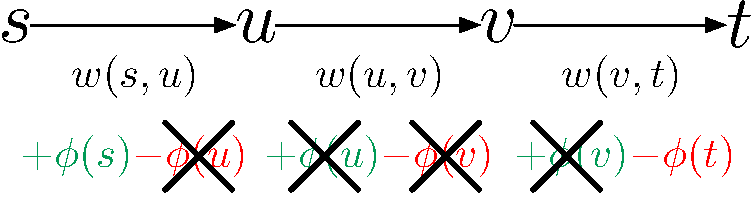
\includegraphics[height=2cm]{images/price2.pdf}
    \caption{Example s-t path. The prices for all `transit' vertices cancel out, and we are left with $\phi(s) - \phi(t)$.}
    \label{fig:price}
\end{figure}
Since all paths between any two vertices $s$ and $t$ are shifted up by the same constant $\phi(s) - \phi(t)$, the shortest paths in the graph remain unchanged! This leads very naturally to the question: \emph{can we use price functions to make all the weights nonnegative, and then just use Dijkstra's?}
\section{Graphs With Only a Few Negative Edges}
\label{sec:fewneg}
The second idea is that if a graph has only \emph{a few} negative edges on any shortest path between two vertices, then we can efficiently compute a price function that makes all the weights in the graph nonnegative.

\begin{definition}[$\eneg(G)$]
    For any weighted graph $G=(V, E, w)$, define
    $$\eneg(G) := \{e \in E | w(e) < 0\}$$
\end{definition}

\begin{definition}[$G_s$]
    Given any graph $G=(V, E, w)$,
    $$G_s = (V \cup \{s\}, E \cup \{(s, v)\}_{v \in V}, w_s)$$ refer to the graph $G$ with a dummy source $s$ added, where there is an edge of weight 0 from $s$ to $v$ for every $v \in V$ and no edges into $s$.
\end{definition}

\begin{definition}[$\eta_G(v), \eta(G)$] \label{def:numberofnegedges}
    For any graph $G=(V, E, w)$, let s be the dummy source in $G_s$. Define
    $$\eta_G(v) := \begin{cases}\infty &\text{if } dist_{G_s}(s, v) = -\infty\\
    min\{|\eneg(G)\cap P|: \text{P is a shortest sv-path in } G_s\}; &\text{otherwise}.\end{cases}$$
    $$\eta(G) = max_{v \in V} \eta_G(v)$$
\end{definition}

\begin{definition}[$dist_i(v)$] \label{def:distwithnegedges}
    For each $v \in V$ and each integer $i \ge 0$, define $dist_i(v)$ to be the weight of a shortest path from $s$ to $v$ among all $s$-to-$v$ paths in G containing at most i edges of $\eneg(G)$. 
\end{definition}

\begin{lemma}[\cite{Johnson77}] \label{lem:distpf}
    Let $G=(V,E)$ be a directed graph with no negative-weight cycle and let s be the dummy source in $G_s$. Let $\phi(v) = dist_{G_s}(s, v)$ for all $v \in V$. Then, all edge weights in $G_\phi$ are non-negative.
\end{lemma}
\begin{proof}
    We have the fact that $dist(s, v) \le dist(s, u) + w(u, v)$. So,
    $$w_\phi(u, v) = w(u, v) + \phi(u) - \phi(v) = w(u, v) + \dist_{G_s}(s, u) - \dist_{G_s}(s, v) \ge 0$$
\end{proof}

\begin{lemma}[$\SPaverage$] \label{lem:elimneg}
    There exists an algorithm $\ElimNeg(G)$ that takes as input a graph $G=(V, E, w)$ in which all vertices have constant out-degree. If $G$ has no negative cycles, the algorithm outputs a price function $\phi$ such that $w_\phi(e) \ge 0$ for all $e \in E$ and has running time $O(\log n \cdot (n + \sum_{u \in V}\eta_G(v)))$.
\end{lemma}

\subsection{Algorithm: Dijkstra + Bellman Ford}

\begin{algorithm2e}[H]
\caption{Algorithm for $\ElimNeg(G)$}
Set $d(s) \gets 0$ and $d(v) \gets \infty$ for $v \neq s$

Initialize priority queue Q and add s to Q.

Initially, every vertex in unmarked.

\tcp*[h]{\textcolor{blue}{Dijkstra Phase}}

\While{Q is non-empty}{
    Let v be vertex in Q with minimum d(v)
    
    Extract v from Q and mark v \\
    
    \ForEach{edge $(v, x) \in E \backslash \eneg(G)$}{
        \If{$d(v) + w(v, x) < d(x)$}{
            add x to Q \tcp*{x may already be marked or in Q.}
            
            $d(x) \gets d(v) + w (v, x)$
        }
    }
}
\tcp*[h]{\textcolor{blue}{Bellman-Ford Phase}}

\ForEach{marked vertex $v$}{
    \ForEach{edge $(v, x) \in eneg(G)$}{
        \If{$d(v) + w(v, x) < d(x)$}{
            Add $x$ to $Q$
            
            $d(x) \gets d(v) + w(v, x)$
        }
    }
    Unmark v
}
If Q is empty: \Return d(v) for each $v \in V$ \tcp*{d(x) does not change so we get final distances.}

Go to Line 4 \tcp*{Q is non-empty.}
\end{algorithm2e}
The priority queue Q is implemented as a binary heap, supporting each queue operation in $O(\log n)$ time. In the following, we say that an edge $(v, x)$ of $G$ is active if $d(v) + w(v, x) < d(x)$ and inactive otherwise.

\subsection{Correctness}
\begin{lemma} \label{lem:dijkstraphase}
    After any execution of the Dijkstra Phase, all edges of $E \backslash \eneg(G)$ are inactive.
\end{lemma}
\begin{proof}
    For iteration i = 0, we run Dijkstra's algorithm on $E \backslash \eneg(G)$, so all edges in $E \backslash \eneg(G)$ become inactive. For iteration $i > 0$, we assume that the lemma is true for iteration $i - 1$. At the end of the Dijkstra phase of iteration $i - 1$, all edges in $E \backslash \eneg(G)$ are inactive. The Bellman Ford phase of iteration $i - 1$ might decrease some of $d(v)$, which will cause some edges in $E \backslash \eneg(G)$ become active. We add these vertex v to Q and execute the Dijkstra phase of iteration $i$, then all edges in $E \backslash \eneg(G)$ will be inactive.
\end{proof}

\begin{lemma}
    After any execution of Bellman-Ford Phase, for any edge $(u, v) \in \eneg(G)$, if $(u, v)$ is active then $u \in Q$.
\end{lemma}
\begin{proof}
    We claim that: if any edge $(u, v) \in \eneg(G)$ is active, $u \in Q$ or $u$ is marked. According to the algorithm, we know that all vertices will be unmarked after Bellman Ford phase. So the lemma can be proved with this claim.
    
    To prove this claim, we consider the situation where the claim might be false. In line 6, we remove $v$ from Q. But we mark it immediately. In line 10 and 15, $d(x)$ is decreased, so some edges $(x, y)$ will become active. But we have already add x to Q in line 9 and 14. In line 16, we unmark $v$. But we decrease $d(v)$ for all active edge $(u, v)$, which makes them inactive. Therefore, the claim stands up.
\end{proof}

\begin{corollary}
    If the algorithm terminates, all edges are inactive.
\end{corollary}

\begin{lemma}
    If $G$ has no negative cycles then after the Dijkstra Phase in iteration $i \ge 0$, $d(v) < dist_i(s, v)$ (Definition \ref{def:distwithnegedges}) for each $v \in V$. 
\end{lemma}
\begin{proof}
    For iteration $i = 0$, the lemma follows from Lemma \ref{lem:dijkstraphase}. For $i > 0$, we assume the lemma holds for iteration $i - 1$. Let $P$ be the shortest path from s to v containing at most $i$ edges of $\eneg(G)$. We assume $P$ has exactly $i$ edges of $\eneg(G)$. Partition $P$ into maximal subpaths $P_0, e_0, P_1, e_1, ..., e_{i-1}, P_i$, where $P_j$ contains only edges from $E \backslash \eneg(G)$ and $e_j \in \eneg(G)$. Let $s_j$ be the first vertex and $t_j$ be the last vertex of subpath $P_j$. Let $j$ be the first iteration where $d(t_i-1) \le dist_{i-1}(s, t_{i-1})$ after the Dijkstra Phase, so $j \le i-1$. Now we want to prove $t_{i-1}$ is marked after the Dijkstra Phase of iteration j. If the Dijkstra Phase of iteration $j$ reduced $d(t_{i-1})$, $t_{i-1}$ is marked. So we assume the opposite situation. Because of the minimality of $j$, $d(t_{i-1})$ is reduced and $t_{i-1}$ is added to $Q$ in the Bellman-Ford Phase of $j-1$. So, $t_{i-1}$ will be extracted from Q and marked in the Dijkstra Phase of iteration j. And the subsequent Bellman-Ford Phase relaxes $(t_{i-1}, s_i)$. Then, we know $d(s_i) \le dist_i(s, s_i)$ at the beginning of iteration $i$. By Lemma \ref{lem:dijkstraphase}, we can get the result $d(v) \le dist_i(s, v)$ after the Dijkstra Phase in iteration $i$.
\end{proof}

\begin{figure}[ht]
    \centering
    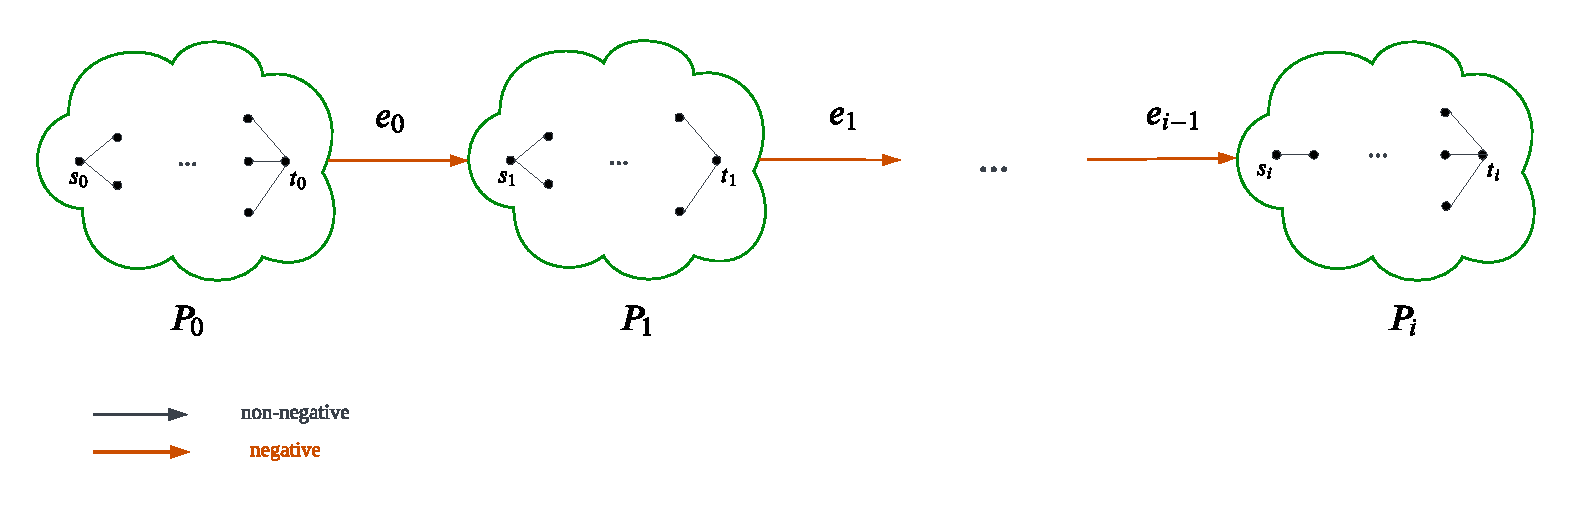
\includegraphics[width=0.9\linewidth]{images/partition.pdf}
    \caption{Partition $P$ into maximal subpaths $P_0, e_0, P_1, e_1, ..., e_{i-1}, P_i$, where $P_j$ contains only non-negative edges and $e_j$ are negative.}
\end{figure}

\begin{corollary}
    If $G$ has no negative cycles, the algorithm terminates with $d(v) = dist(s, v)$ for each $v \in V$.
\end{corollary}

\subsection{Runtime}
By assumption, all vertices in G have constant out-degree. For vertex extracted from Q in Dijkstra Phase and for marked vertex processed in Bellman-Ford Phase, there are only a constant number of outgoing vertex. So, the dominant part of running time is the update of Q.

Each vertex $v$ is added to Q at most once in each of Dijkstra and Bellman Ford phrase per iteration. If $dist(s, v) = dist_i(s, v)$, v is added to Q $O(i+1)$ times and $d(v) = dist(s, v)$ after the Dijkstra Phase of the $(i+1)$th iteration. After that, $d(v)$ will not change and vertex $v$ will not be added to Q. Here we know $dist(s, v) = dist_{\eta_{G}(v)}(s, v)$, so v is added to Q $O(\eta_G(v) + 1)$ times. For all $v \in V$, the overall time added to Q is $O(\sum_{v \in V}(\eta_G(v)+1)) = O(n + \sum_{v \in V}\eta_G(v))$. In addition, the number of extractions from Q cannot exceed the number of insertions. The priority queue Q is implemented as a binary heap, so each queue operation takes $O(\log n)$ time. Therefore, the running time of the algorithm is $O(\log(n) \cdot (n + \sum_{u \in V}\eta_G(v)))$.

\section{Low Diameter Decomposition (LDD)}
\label{sec:ldd}
In section \ref{sec:fewneg} we saw how we can efficiently compute price functions if the graph we are given has a constant number of negative edges on any shortest path. But it is not yet clear how to deal with the general case where there might be $O(n)$ negative edges along any shortest path. The third main idea we will discuss in this lecture is a decomposition for directed graphs which partitions the vertices into subsets each of which have low `weak diameter'. 

\begin{definition}{Weak Diameter}

    Given a directed graph $G = (V, E, w)$, we say that a subset $S \subseteq V$ has \emph{weak diameter $D$} iff:
    $$\forall u, v \in S, d_G(u,v) \leq D$$
\end{definition}

\begin{definition}{Low Diameter Decomposition (LDD)}
         \begin{tight_itemize}
             \item \textbf{Input:} A graph $G$ with non-negative edge weights, and a \emph{non-negative} integer $D$
             \item \textbf{Output:} A set of edges \textcolor{black}{$\esep$} such that the strongly connected components (SCCs) $V_1, \dots, V_k$ of $G - \esep$ have weak diameter $D$ in $G$
         \end{tight_itemize}
\end{definition}
\begin{figure}[ht]
    \centering
    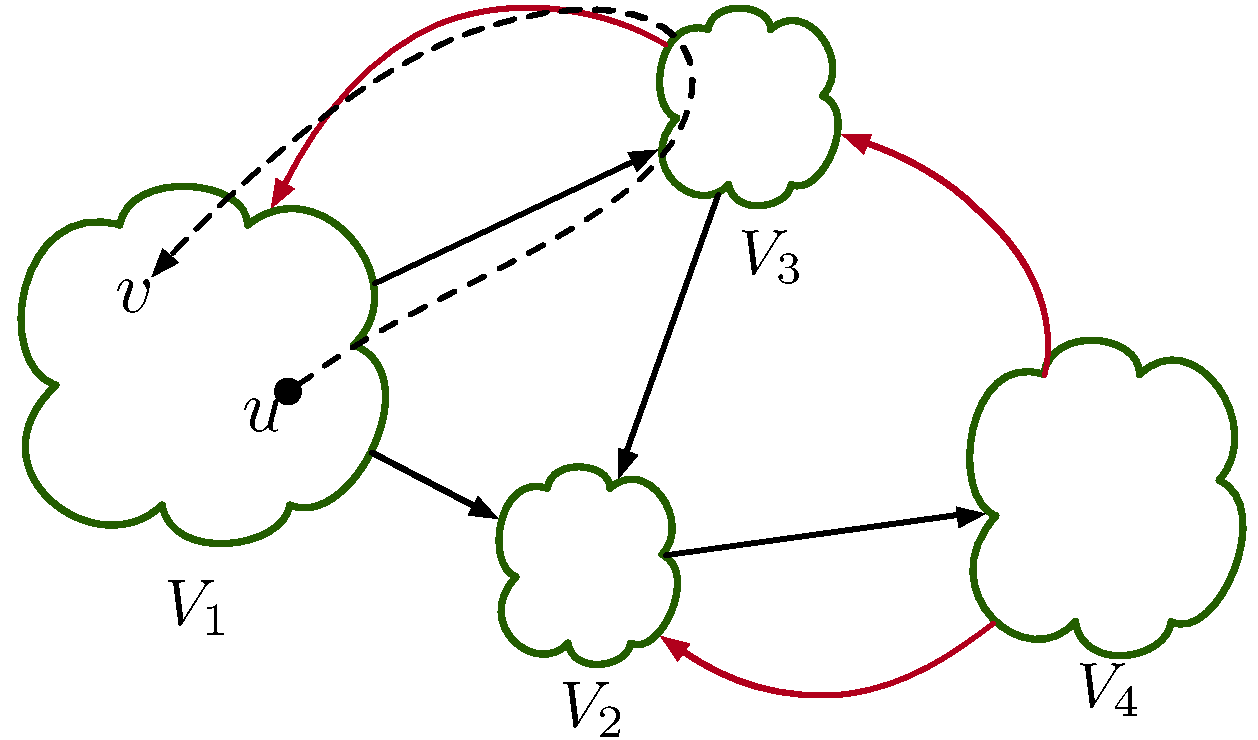
\includegraphics[width=0.4\linewidth]{images/ldd.pdf}
    \caption{A depiction of the output of LDD. The edges in $\esep$ are depicted in red, and the green bubbles represent the SCCs of $G - \esep$. Each of these SCCs $\{V_1, V_2, V_3, V_4\}$ are guaranteed to have weak diameter $D$ in the original graph.}
    \label{fig:my_label}
\end{figure}

\begin{lemma} \label{lem:ldd}
    There exists an algorithm $\LowDiamDecomposition(G, D)$ which computes the LDD in  $O(m\log^2 n+n\log^3 n)$ time and guarantees that:
    $$\forall e \in E, \Pr[e \in \textcolor{black}{\esep}] = O\left(\frac{w(e) \cdot \log^2 n}{D} + n^{-10}\right)$$
\end{lemma}

 We will not prove lemma \ref{lem:ldd} in this lecture. The basic mechanism of $\LowDiamDecomposition(G, D)$ is to recursively carve out balls around each vertex until the balls become singletons or have low diameter. In addition to the algorithm and proofs given in the paper, we refer the reader to these additional notes by one of authors \cite{LDD}.

\section{Overview of $\ScaleDown$ Algorithm}
We now have most of the tools we need to describe the main workhorse of the approach, which is a recursive algorithm called $\ScaleDown$ that takes
a graph with edge weights $w(u,v) \geq -2B$ for some positive integer $B$ and returns a price function $\phi$ such that $w_\phi(u,v) \geq -B$.

Given a graph $G$, $\ScaleDown$ operates on a slightly modified version of the graph, denoted $\GB$, in which all the negative weights are shifted up by the constant $B$. Note $\GB$ may still have negative edges, so we also define $\GB_{\geq 0}$ in which any weights that remain negative are rounded up to 0.
\begin{definition}{$\GB, \GB_{\geq 0}, \GB_s$}

    $\GB:=(V, E, \wB)$  where $\wB(e) := w(e) + B$ if $w(e) < 0$

    $\GB_{\geq 0}:=(V, E, \wB_{\geq 0})$ where $\wB_{\geq 0}(e) := \max \{0, \wB(e) \}$

\end{definition}


\begin{theorem}[$\ScaleDown$]
\label{thm:scaledown}
There exists the following algorithm $\ScaleDown(G = (V,E,w),\Delta,B)$.
\begin{tight_enumerate}
    \item \textbf{Input Requirements:} \label{item:ScaleDown input}
    \begin{tight_enumerate}
        \item\label{prop:scaledown:weight} $B$ is positive integer, and $w(e) \geq -2B$ for all $e \in E$
        \item\label{prop:scaledown:Delta} 
        for every $v \in V$  
        %$\max_{v\in V}\eta_{G^{B/2}}(v) \leq \Delta$ 
        there is a shortest $sv$-path in $\GB_s$ with at most $\Delta$ negative edges \label{item:ScaleDown input b}
    \end{tight_enumerate}
    \item \label{item:ScaleDown Output} \textbf{Output:} $\phi$ such that $w_{\phi}(e) \geq -B$ for all $e \in E$
    \item \textbf{Run Time:}\label{item:ScaleDown Runtime} expected runtime $O\left(m\log^3(n)\log(\Delta)\right)$.
\end{tight_enumerate}

\end{theorem}

\begin{algorithm2e}[H]
% \captionsetup{labelformat=empty}
\caption{$\ScaleDown(G = (V,E,w),\Delta,B)$}\label{alg:ScaleDown}

\If{$\Delta\leq 2$}{
 \label{line:ScaleDown:BaseCase}
    \Return $\SPaverage(\GB)$

}


%   Let $d=\Delta/2$. 



\BlankLine

\tcp*[h]{\textcolor{blue}{Phase 0: Decompose $V$ to SCCs $V_1, V_2, \ldots$ }}\\
\tcp*[h]{\textcolor{blue}{with weak diameter $\frac{\Delta B}{2}$ in $\GB_{\geq 0}$}}


$\esep \gets \SCCDecomposition(\GB_{\geq 0}, \frac{\Delta B}{2})$ %(\Cref{lem:SCCDecomposition})
\label{line:ScaleDown:LowDiamDecomposition}

% Compute Strongly Connected Components (SCCs) of $\GB \setminus \esep$, denoted by $V_1, V_2, \ldots$ \label{line:ScaleDown:SCC decomposition} \\ \tcp*[h]{Properties: (\Cref{thm:ScaleDown:Weak Diameter}) For each $u,v\in V_i$, $\dist_G(u,v)\leq dB$.} \\ \tcp*[f]{(\Cref{thm:ScaleDown:expected esep}) If $\eta(\GB)\leq \Delta$, then for every $v\in V_i$, $E[P_{\GB}(v)\cap \esep]=O(\log^2 n)$}


\BlankLine


\tcp*[h]{\textcolor{blue}{Phase 1: Make edges inside the SCCs $\GB[V_i]$ non-negative}}


$\phi_1\gets \ScaleDown(\bigcup_i G[V_i], \Delta/2, B)$ \label{line:ScaleDown:Recursion}% \tcp*[f]{(\Cref{thm:ScaleDown:Phase 1 conclusion}) $w_{H^B_{\phi_1}}(e)\geq 0$ for all $e\in H$}

\BlankLine



\tcp*[h]{\textcolor{blue}{Phase 2: Make all edges in $\GB \setminus \esep$ non-negative}} 


$\phi_2 \gets \phi_1 + \FixAlmostDag(\GB_{\phi_1} \setminus \esep, \{V_1, V_2, \ldots \})$ %(\Cref{lem:almostDag}) \label{line:ScaleDown:callFixAlmostDAG} 


% $\phi_{2} \gets \phi_1 + \psi$ % \tcp*[f]{(\Cref{thm:ScaleDown:Phase 2 conclusion}) All edges  in $(\GB \setminus \esep)_{\phi_2}$ are non-negative} 


\BlankLine


\tcp*[h]{\textcolor{blue}{Phase 3: Make all edges in $\GB$ non-negative}}

$\phi_3 \gets \phi_2+\SPaverage(\GB_{\phi_2})$ % \tcp*[f]{(\Cref{thm:ScaleDown:main output correctness}) All edges in $\GB_{\phi_3}$ are non-negative.} 


\Return $\phi_3$ %\tcp*{Since $\wB_{\phi_3}(e)\geq 0$, we have $w_{\phi_3}(e)\geq -B$}


\end{algorithm2e}

\subsection{Runtime}
\label{sec:scaledownruntime}
ScaleDown operates recursively, using $\Delta$ as its recursion parameter. When $\Delta \leq 2$, it simply calls $\SPaverage$, which we already analyzed in section \ref{sec:fewneg}. Since $\Delta \leq 2$ this base case is $O(n \cdot \log(n))$.

Before the recursion, we compute LDD as described in section {sec:ldd} on the graph in $\GB_{\geq 0}$ in $O(m\log^2 n+n\log^3 n)$ time, and after the recursion, we call $\FixAlmostDag$ which we will see later takes $O(m + n)$ time.

Before returning, we call $\SPaverage$ to fix the edges in $\esep$. Since those are the only edges that remain negative after the previous two steps, and because the probability that any edge in the graph is in $\esep$ is bounded (from the low diameter decomposition), we will show that this step has expected runtime $O(m \log^3 m)$.

From the pseudocode, we see that the recursive step halves the value of $\Delta$ at each level (we will see why in the next section), so there can only be $\log(\Delta)$ levels to this recursion. Putting this all together, we get a total runtime of $O\left(m \log^3 (m) \log \Delta \right)$.

\section{Phase 1: Pricing Edges Inside SCCs}
By the input requirements of $\ScaleDown$, the graph $\GB$ is guaranteed to have at most $\Delta$ negative edges along any sv shortest path.
We will now show that within each of the SCCs that we obtain from the low diameter composition in Phase 0 of $\ScaleDown$, the value of this parameter is reduced to $\frac{\Delta}{2}$.
Note that this is necessary for the correctness of the algorithm, since Phase 1 of $\ScaleDown$ is a recursive call that requires this property of its input graph.

\begin{lemma}
    For all $v \in V_i$, we have \textbf{at most $\frac{\Delta}{2}$ negative edges} on the shortest $sv$-path in $G[V_i]^B_s$.
\end{lemma}

\begin{wrapfigure}{r}{5cm}
    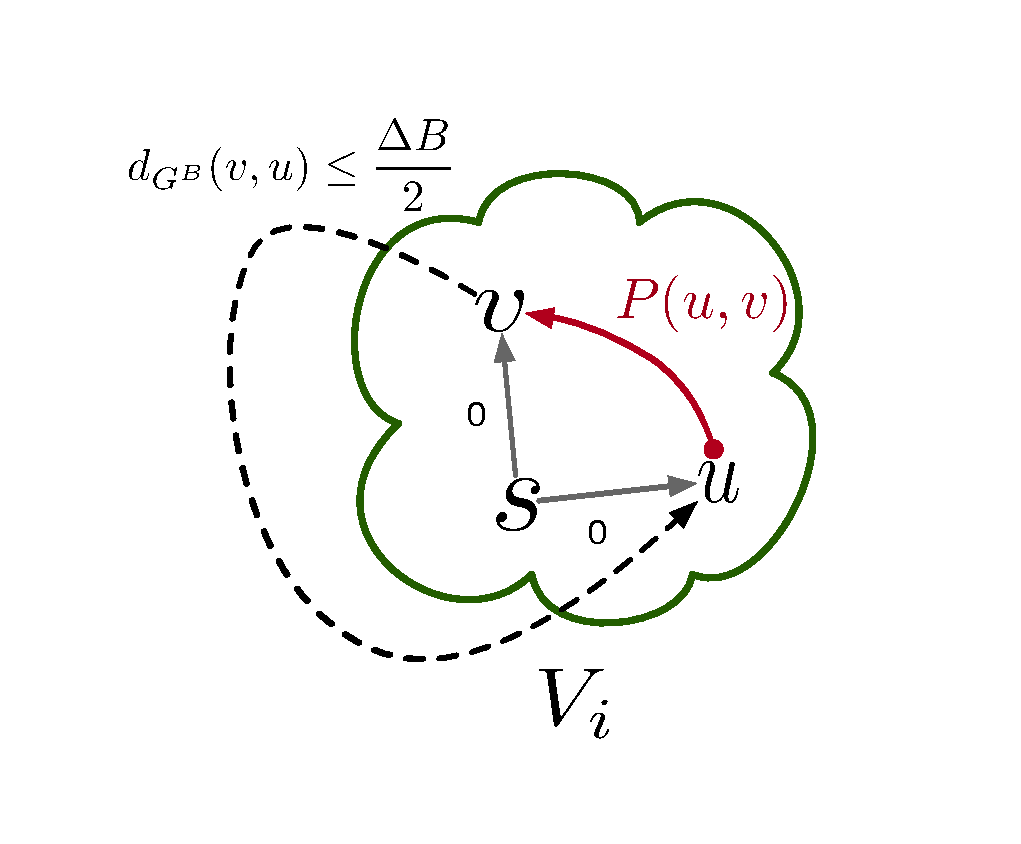
\includegraphics[width=5cm]{images/phase1-2.pdf}
\end{wrapfigure}
\textit{Proof.} Consider one of the SCCs, $V_i$. Let $P(s,v)$ be the shortest $sv$-path in $G[V_i]^B_s$.

Let $u$ be the first vertex along $P(s,v)$. If there is no such $u$, then the path $P(s,v)$ contains a single zero weight edge from $s$ to $v$ and the claim is trivially true. On the other hand, if there is such a $u$, then we know that the path from u to v $P(u,v)$ must have non-positive weight.

$$w_B(\textcolor{black}{P(u,v)}) \leq 0$$

Let $k$ be the number of negative edges in $\textcolor{black}{P(u,v)}$. If we compare the weight in $\GB$ to the weight in $G$, we must have: 

$$w(\textcolor{black}{P(u,v)}) \leq w_B(\textcolor{black}{P(u,v)}) -B \cdot k \leq  -B \cdot k$$

From LDD, we have $d_{\GB} (v, u) \leq  \frac{\Delta B}{2}$. This is depicted as the dotted arrow in the figure on the right.

    $$d_G(u,v) \leq d_{\GB} (v, u) \leq  \frac{\Delta B}{2}$$

Since these two paths form a cycle, and we know there are no negative cycles, we must have:
    $$0 \leq d_G(v,u) + w(\textcolor{black}{P(u,v)})$$

    $$0 \leq d_G(v,u) + w(\textcolor{black}{P(u,v)}) \leq  \frac{\Delta B}{2} -B \cdot k$$
$$k \leq \frac{\Delta}{2} $$





    
\section{Phase 2: Pricing DAG Edges}
All edges in $G^B_{\phi_1}[V_i]$ become non-negative after phase 1, so we turn to the remaining edges in $G^B \backslash \esep$. After contracting every $V_i$ into a node, the resulting graph with remaining edges is a directed acyclic graph (DAG). We introduce Lemma $\FixAlmostDag$, calling it with $G=G^B_{\phi_1} \backslash \esep$ and $P = \{V_1, V_2, \dots\}$. As a result, it returns $\varphi$ such that $(G^B_{\phi_1} \backslash \esep)_\varphi = G^B_{\phi_2} \backslash \esep$ contains no negative-weight edges.

\begin{lemma}
There exists an algorithm $\FixAlmostDag(G, P)$ that takes as input a graph $G$ and a partition $P := {V_1, V_2, ...}$ of vertices of G such that
\begin{enumerate}
    \item for every i, the induced subgraph $G[V_i]$ contains no negative-weight edges, and
    \item when we contract every $V_i$ into a node, the resulting graph is a DAG(i.e. contains no cycle).
\end{enumerate}
The algorithm outputs a price function $\phi$: $V \to \mathbb{Z}$ such that $w_\phi(u, v) \ge 0$ for all $(u, v) \in E$. The running time is $O(m+n)$.
\end{lemma}


\begin{algorithm2e}[H]
\caption{$\FixAlmostDag(G=(V, E, w), P=\{V_1, V_2, ...\}$}

Relabel the sets $V_1, V_2, ...$ so that they are in topological order in G. That is, after relabeling, if $(u, v) \in E$, with $u \in V_i$ and $v \in V_j$, the $i \le j$.

Define $\mu_j = min\{w(u, v) | (u, v)\} \in \eneg(G), u \notin V_j, v \in V_j$; here, let $min{\varnothing} = 0$.

\tcp*[h]{$\mu_j$ is min negative edge weight entering $V_j$, or 0 if no such edge exists.}

Define $M_1 \gets \mu_1 = 0$.\\

\For(\tcp*[f]{make edges into each $V_2, \dots, V_q$ non-negative}){$j = 2$ to q}{ 
$M_j \gets M_{j-1} + \mu_j$; \tcp*{$M_j = \sum_{k \le j}\mu_k$}

Define $\phi(v) \gets M_j$ for every $v \in V_j$
}

\Return{$\phi$}
\end{algorithm2e}

\begin{figure}[ht]
    \centering
    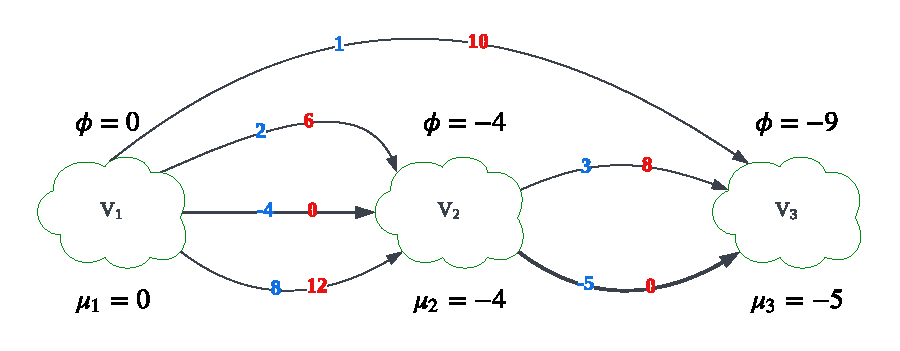
\includegraphics[width=0.9\linewidth]{images/phase2.pdf}
    \caption{Algorithm $\FixAlmostDag$ on an example graph $G$. After computing $\mu_j$ for each component $V_j$ and price function $\phi(v)$ for each $v \in V_j$, all edge weights in $G^B_{\phi_2} \backslash \esep$ become non-negative.}
\end{figure}

For line 2, each $\mu_j$ requires $O(1)$ + [number of edges entering $V_j$]. Because the $V_j$ are disjoint, the total time to compute all $\mu_j$ is $O(m + n)$. For loop in line 4, we only consider each vertex once, so the total time is $O(n)$. The overall running time is $O(m+n)$.

\begin{proof}
We need to show $w_\phi(u, v) \ge 0$ for all $(u, v) \in E$.
Say that $u \in V_i$ and $v \in V_j$. Because the sets are in topological order, we have $i < j$. By definition of $\mu_j$, we have $\mu_j < w(u, v)$. Therefore, we have
$$w_\phi(u, v) = w(u, v) + \phi(u) - \phi(v) = w(u, v) + M_i - M_j = w(u, v) - \sum_{k=i+1}^{j}\mu_k \ge w(u, v) - \mu_j  \ge 0 $$
\end{proof}

\section{Phase 3: Pricing Separator Edges}
The only negative edges remaining are in $\esep$. By lemma \ref{lem:distpf}, we can set price function $\phi(v) = dist_{G_s}(s, v)$ to make all edge weights non-negative. By lemma \ref{lem:elimneg}, we can compute all distances in $O(\log n \cdot (n + \sum_{u \in V}\eta_G(v)))$. Since we assume every vertex in $G$ has constant out-degree, $m = \Theta(n)$. So, we can use $m$ and $n$ interchangeably. The running time become $O(\log m \cdot (m + \sum_{u \in V}\eta_G(v)))$.

Now, we want to prove for any $v \in V$, $\E[\eta_{\GB_{\phi_2}}(v)] = O(\log^2 m)$.

\begin{lemma} \label{lem:pathwitherem}
    If $\eta(\GB) \le \Delta$, then for every $v \in V$, $E[|P_\GB(v) \cap \esep|] = O(\log^2 m)$ ($\eta(\GB)$ from Definition \ref{def:numberofnegedges}).
\end{lemma}

\begin{proof}
    By decomposition, the path can be divided to negative and non-negative parts:
    $$\wB_s(P_\GB(v)) = \wB_{\ge 0}(P_\GB(v)) + \wB_{<0}(P_\GB(v))$$
    In $\GB_s$, the $\wB_s(P_\GB(v))$ as the path length must be less than or equal to the edge weight from s to v. By definition of $G_s$, the edge weight is 0 from s to every $v \in V$. So,
    $$\wB_s(P_\GB(v)) \le 0$$
    Recall the input of $\ScaleDown$ (Theorem \ref{thm:scaledown}) that $w(e) \ge -2B$. By adding $B$ to all negative edges, $\wB(e) \ge -B$ for all $e \in E$. So,
    \begin{align*}
        \wB_{<0}(P_{\GB}(v)) &= \sum_{e \in P_{\GB}(v) \cap \eneg(\GB)} \wB(e)\\
        &\ge |P_{\GB}(v) \cap \eneg(\GB)| \cdot (-B)\\
        &= \eta_{\GB}(v) \cdot (-B)\\
        \wB_{\ge 0}(P_{\GB}(v)) &= \wB_s(P_{\GB}(v)) - \wB_{<0}(P_{\GB}(v))\\
        &\le \eta_{\GB}(v) \cdot B
    \end{align*}
    Recall the output of $\LowDiamDecomposition$ (Lemma \ref{lem:ldd}) that $\Pr[e \in \esep] = O(\frac{\wB_{\ge 0}(e) \cdot \log^2 n}{D} + n^{-10})$, and we have $D=dB=B\frac{\Delta}{2}$. So,
    \begin{align*}
        \E[P_{\GB}(v) \cap \esep] &= O(\frac{\wB_{\ge 0}(P_\GB(v)) \cdot \log^2 n}{B\frac{\Delta}{2}} + |P_{\GB}(v)| \cdot n^{-10})\\
        &=O(\frac{2\eta_{\GB}(v) \cdot \log^2 n}{\Delta} + n^{-9})
    \end{align*}
    If $\eta(\GB) \le \Delta$,
    $$\E[P_{\GB}(v) \cap \esep] = O(\log^2 n)$$
\end{proof}

Now we are ready to compute the expected runtime of $\ElimNeg(\GB_{\phi_2})$ in Phase 3. Note that, regardless of the value of $\phi_2$, $P_{\GB}(v)$ is a shortest sv-path in $\GB_{\phi_2}$ for any $v \in V$. By Definition \ref{def:numberofnegedges},
\begin{align*}
    \eta_{\GB_{\phi_2}} &= min\{|P \cap \eneg(\GB_{\phi_2}|: \text{P is a shortest sv-path in } (\GB_{\phi_2})_s\}\\
    &\le |P_{\GB(v)} \cap \eneg(\GB_{\phi_2}|
\end{align*}

The only negative edges remaining are in $\esep$, which means $\eneg(\GB_{\phi_2}) \subseteq \esep$. So,
$$\eta_{\GB_{\phi_2}}(v) \le |P_{\GB(v)} \cap \esep|$$

By Lemma \ref{lem:pathwitherem} and the input of Theorem \ref{thm:scaledown} that $\eta(\GB) \le \Delta$,
$$\E[\eta_{\GB_{\phi_2}}(v)] \le \E[|P_{\GB(v)} \cap \esep|] = O(\log^2 m)$$
Therefore, the expected runtime of $\ElimNeg(\GB_{\phi_2})$ in Phase 3 is
$$O\left(\log m \cdot \left(m + \E\left[\sum_{u \in V}\eta_G(v)\right]\right)\right) = O(m \log^3 m)$$


\section{Putting it all Together}
Now that we have our $\ScaleDown$ operation which can take a graph with $w(e) \geq -2B$ and returns a price function such that $w_\phi \geq B$, it only remains to show how this can be used to solve the shortest path problem. The idea is to scale all the weights of the input graph up by $2n$, then use ScaleDown $\log 2n$ times to compute a price function which brings all the weights back up to $w(e) \geq -1$. Then we simply add 1 to all weights and call Dijkstras on the resulting graph $G^\star$ which will have strictly nonnegative weights. 

\begin{algorithm2e}[H] 
\caption*{$\SPmain(\gin,\sin)$}	\label{alg:SPmain}

\tcp*[h]{scale up edge weights}

$\wbar(e) \gets \win(e) \cdot 2n$ 

$B \gets 2 n$


\For(\label{line:SPMain:ForLoop}){$i = 1$ to $t:=\log_2(B)$}{

$\psi_i \gets \ScaleDown(\Gbar_{\phi_{i-1}},\Delta := n,B/2^{i})$ \label{line:SPMain:callScaleDown} 

$\phi_i \gets \phi_{i-1}+\psi_i$ 

\tcp*[h]{$w_{\phi_i}(e)\geq -B/2^{i}$ }
\label{line:SPMain:endForLoop} 

}


$\wstar(e) \gets \wbar_{\phi_t}(e) + 1$ 


\tcp*[h]{Observe: $\Gstar$ in above line has non-negative weights}



$T \gets \Dijkstra(\Gstar, s_{in})$  \label{line:SPMain:callDijkstra} 

\Return shortest path tree $T$ \label{line:SPMain:Dijkstragstar}. 

\end{algorithm2e}

\subsection{Correctness}
It should be clear that scaling the weights up by $2n$ from $w(e)$ to $\bar w(e)$ will not change the shortest path. And we have seen that modifying the weights using price functions also preserves shortest paths. Since $\wbar_{\phi_t}(e) $ differs from $\bar w(e)$ only via price functions, it only remains to show that adding 1 to $\wbar_{\phi_t}(e) $ to obtain $\wstar(e) $ will not change the shortest path.

To see why this is the case, consider any two vertices $s, t \in V$. As we have seen in \ref{sec:price} the cost of all s-t paths under
$\wbar_{\phi_t}$ are shifted by the same constant $\phi(s) - \phi(t)$. Therefore, the difference in cost between any s-t paths is the same under 
$\wbar_{\phi_t}$ and $\bar w$. Since we scaled all edge weights up by $2n$ to obtain $\bar w$, no two s-t paths can differ by less than $2n$. But, adding 1 to all edges can only increase the cost of any path by $(n-1)$ since there are at most $(n-1)$ edges in a path with no cycles. 

 \subsection{Runtime}
We saw in section \ref{sec:scaledownruntime} that the running time of a single call to $\ScaleDown$ will be $O\left(m \log^3 (m) \log \Delta \right)$. In algorithm \ref{alg:SPmain}, there are $O(\log n)$ calls to $\ScaleDown$ with $\Delta = n$ so the total runtime is $O\left(m \log^5 (m) \right)$. 

\printbibliography
\end{document}
